% !TeX spellcheck = en_US
\documentclass[french]{yLectureNote}

\title{Électrocinétique}
\subtitle{Physique}
\author{Paulhenry Saux}
\date{\today}
\yLanguage{Français}

\professor{Allard}%allard@irsamc.ups-tlse.fr
\usepackage{graphicx}%----pour mettre des images
\usepackage[utf8]{inputenc}%---encodage
\usepackage{geometry}%---pour modifier les tailles et mettre a4paper
%\usepackage{awesomebox}%---pour les boites d'exercices, de pbq et de croquis ---d\'esactiv\'e pour les TP de PC
\usepackage{tikz}%---pour deiffner + d\'ependance de chemfig
\usepackage{tkz-tab}
\usepackage{chemfig}%---pour deiffner formules chimiques
\usepackage{chemformula}%---pour les formules chimiques en \'equation : \ch{...}
\usepackage{tabularx}%---pour dimensionner automatiquement les tableaux avec variable X
\usepackage{awesomebox}%---Pour les boites info, danger et autres
\usepackage{menukeys}%---Pour deiffner les touches de Calculatrice
\usepackage{fancyhdr}%---pour les en-t\^ete personnalis\'ees
\usepackage{blindtext}%---pour les liens
\usepackage{hyperref}%---pour les liens (\`a mettre en dernier)
\usepackage{caption}%---pour la francisation de la l\'egende table vers Tableau
\usepackage{pifont}
\usepackage{array}%---pour les tableaux
\usepackage{lipsum}
\usepackage{yFlatTable}
\usepackage{multicol}
\newcommand{\Lim}[1]{\lim\limits_{\substack{#1}}\:}
\renewcommand{\vec}{\overrightarrow}
\begin{document}

	\chapter{Lois de base en régime continu}
\section{Puissance et mode de fonctionnement}
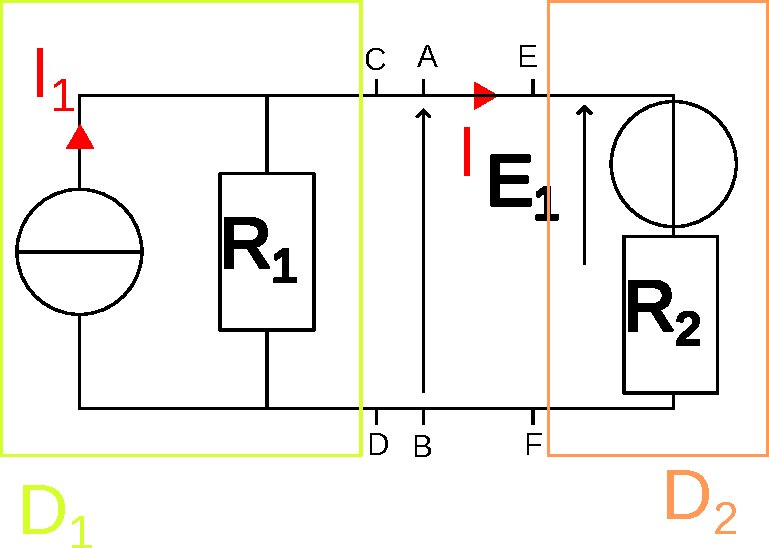
\includegraphics[scale=0.4]{path23}

On cherche à déterminer les puissances associées au dip\^oles D1 et D2. On sait que le circuit fonctionne avec U = 6V et I = 0.5A.

On calule la puissance avec $P=U\times I$. Il faut donc obtenir la tension et ainsi que l'intensité (le courant) qui traversent D1. On introduit pour cela 2 points $C$ et $D$ placés à l'entrée et à la sortie de $D_1$. On remarque que la tension entre ces deux points est la m\^eme qu'entre $A$ et $B$, donc $u=U_{D_1} = U$. Au point $C$ un courant $i$ arrive et repart au point $D$. $I = i$.

La puissance vaut donc $P = U_{AB}i$.

On remarque que dans $D_1$, $\vec{U_{AB}}$ est dans le m\^eme que celui du courant traversant le dip\^ole. On en déduit que $D_1$ est en convention générateur. Il va donc perdre de la puissance pour en fournir au circuit. Sa puissance sera donc négative.\marginCritical{Pour trouver le signe de la puissance, on étudie non pas l'effet du dipole sur le circuit, mais ce qui se passe dans le dip\^ole. Ici, comme le dip\^ole fournit de l'énergie, lui en perd, d'où une puissance négative.}

De la m\^eme manière, on introduit pour cela 2 points $E$ et $F$ placés à l'entrée et à la sortie de $D_2$. On remarque que la tension entre ces deux points est la m\^eme qu'entre $A$ et $B$, donc $u=U_{D_2} = U$\marginTips{On peut le vérifier. Il y a un générareur de tension 3V en série avec une résistance de 6$\omega$. La tension de la résistance vaut $U=RI = 6\times 0.5 = 3$, donc $U_{D_2} = 3 + 3 = 6$V, ce qui correspond à $U$}. Au point $E$ un courant $i$ arrive et repart au point $f$. $I = i$.

La puissance vaut donc $P = U_{AB}i$.

On remarque que dans $D_2$, $\vec{U_{AB}}$ est dans le sens contraire au courant traversant le dip\^ole. On en déduit que $D_1$ est en convention récepteur. Il va donc gagner de la puissance pour fonctionner. Sa puissance sera donc positive.
\section{Loi des noeuds / loi des mailles}
\subsection{Loi des noeuds}
On peut utiliser la loi des noeuds pour trouver des relations entre différents courants en un point. Par exemple, si un courant $i_1$ arrive en un point et deux courants $i_2$ et $i_3$, alors $i_1-i_2-i_3 = 0\iff i_1 = i_2+i_3$
\subsection{Loi des mailles}
On peut utiliser la loi des mailles pour trouver des relations entre la tension de différents dip\^oles.

\warningInfo{Résistances}{En présence de résistance, on peut facilement combiner ces 2 lois en utilisant la relation $U=R\times I$.}
\section{Exemple V)}
On se trouve dans la situation suivante :

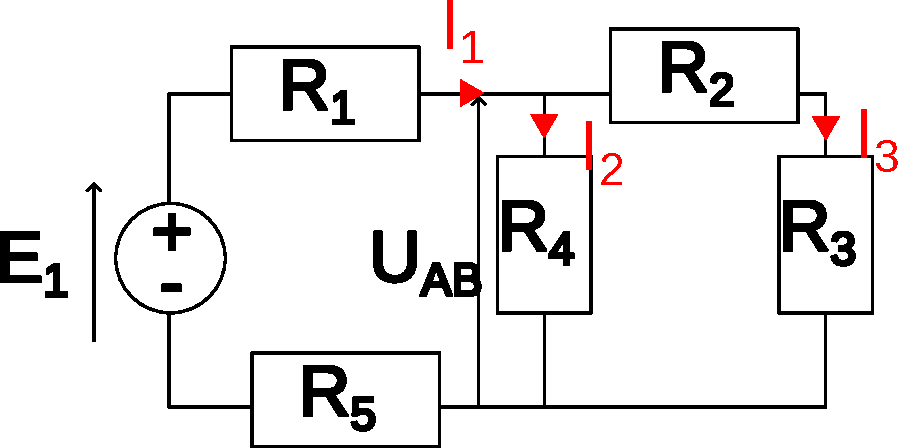
\includegraphics[scale=0.4]{path2}

On cherche à exprimer la tension aux bornes du générateur en fonction de $I_1$ et des résistances.

On va d'abord simplifier le circuit en introduisant $R_A$ la résistance équivalente à $R_1$ et $R_5$ et $R_B$ la résistance équivalente à $R_2$ et $R_3$. En appliquant les formules de résistance en série, on obtient $R_A = R_2 + R_3$ et $R_B = R_1+R_5$.\marginTips{Comme les 2 résistances équivalentes sont des équivalences de résistances en séries, le courant qui passe par la résistance équivalente est le m\^eme qui passe dans les 2 résistances originelles.}

On obtient le schéma suivant :

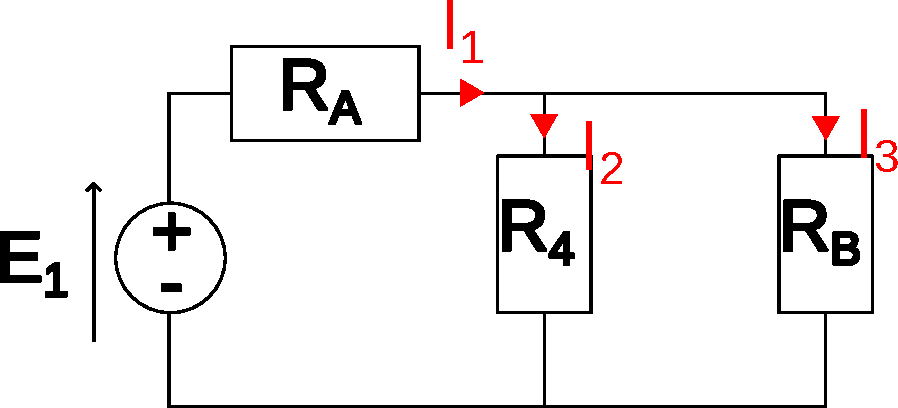
\includegraphics[scale=0.5]{path1}

On peut exprimer la relation entre les courants aux points $A$ et $B$. On a $I_1 = I_2+I_3$.
\explanation{ex_5}{En effet, $I_2 = \frac{U_4}{R_4}$ et $I_3 = \frac{U_B}{R_B}$}
On va maintenant exprimer les courants traversants chaque dip\^ole en fonction de $I_1$ et des résistances. D'après l'expression précédente, on a $I_1 = \frac{U_4}{R_4} + \frac{U_B}{R_B}$.\explain{ex_5}{right}{0}{0.5}{}

Il faut ensuite remarquer que $U_4 = U_B = U_{AB}$. Avec cette nouvelle égalité, on va pouvoir exprimer $U_{AB}$ en fonction de $I_1$ et des résistances. En effet, on a
\begin{flalign*}
I_1 &= \frac{U_{AB}}{R_4} + \frac{U_{AB}}{R_B}\\
&= \frac{U_{AB}(R_4+R_B)}{R_4R_B}\\
U_{AB} &= I_1\frac{R_4R_B}{R_4+R_B}
\end{flalign*}

On peut maintenant exprimer les courants $I_2$ et $I_3$ en fonction de $I_1$ et des résistances :
\begin{flalign*}
I_2 &= \frac{U_{AB}}{R_4}\\
&= I_1\frac{R_B}{R_4+R_B}\\
I_3 &= \frac{U_{AB}}{R_B}\\
&= I_1\frac{R_4}{R_4+R_B}
\end{flalign*}

En appliquant la loi des mailles à celle qui contient le générateur, on obtient cette égalité : $E_1-U_A-U_4 = 0$ où l'on peut remplacer $U_A$ et $U_4$ par leurs expression :

\begin{flalign*}
E_1 &= U_A + U_4\\
& = R_1\times I_1 + R_4\times I_2\\
\end{flalign*}

Ainsi, en connaissant uniquement $I_1$ et les valeurs des résistances, on peut calculer la valeur de $E_1$.
\end{document}

